\chapter{Introduction to Graph Theory}

\section{Introduction}

A graph consists of a nonempty set \(V\)  of vertices and a set E of edges, where each edge in \(E\)  connects two (may be the same) vertices in \(V\). We usually use \(G = (V, E)\) to indicate the above relationship.

\subsection{Simple Graph}
If each edge connects two different vertices, and no two edges connect the same pair of vertices, then the graph is a simple graph. For example, the graph on the left is a simple graph, and the graph on the right is not a simple graph.

\begin{figure}[H]
  \centering
  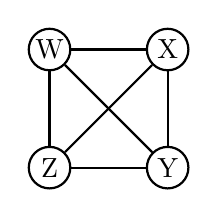
\begin{tikzpicture}[node distance={15mm}, thick, main/.style = {draw, circle}]
    \centering
    \tikzstyle{vertex}=[circle,draw=black,thick,fill=white,minimum size=15pt, inner sep=0pt]
    \node[vertex] (Z) at (0, 0) {Z};
    \node[vertex] (W) at (0, 1.5) {W};
    \node[vertex] (X) at (1.5, 1.5) {X};
    \node[vertex] (Y) at (1.5, 0) {Y};
    \path
    (Z) edge (W) 
    (W) edge (X) 
    (X) edge (Y) 
    (Y) edge (Z)
    (W) edge (Y)
    (Z) edge (X)
    ;
  \end{tikzpicture}
  \quad\quad\quad
  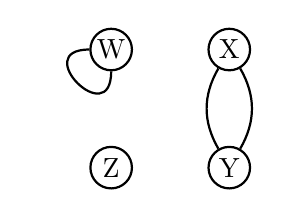
\begin{tikzpicture}[node distance={15mm}, thick, main/.style = {draw, circle}]
    \centering
    \tikzstyle{vertex}=[circle,draw=black,thick,fill=white,minimum size=15pt, inner sep=0pt]
    \node[vertex] (Z) at (0, 0) {Z};
    \node[vertex] (W) at (0, 1.5) {W};
    \node[vertex] (X) at (1.5, 1.5) {X};
    \node[vertex] (Y) at (1.5, 0) {Y};
    \path
    (W) edge [out=180,in=270,looseness=5] (W)
    (X) edge [bend left] (Y)
    (X) edge [bend right] (Y)
    ;
  \end{tikzpicture}
\end{figure}


\subsection{Directed Graph}
A directed graph G consists of a nonempty set \(V\)  of vertices and a set \(E\)  of directed edges, where each edge is associated with an ordered pair of vertices. We write \(G = (V, E)\) to denote the graph. For example

\begin{figure}[H]
  \centering
  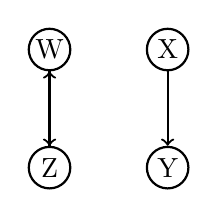
\begin{tikzpicture}[node distance={15mm}, thick, main/.style = {draw, circle}]
    \centering
    \tikzstyle{vertex}=[circle,draw=black,thick,fill=white,minimum size=15pt, inner sep=0pt]
    \node[vertex] (Z) at (0, 0) {Z};
    \node[vertex] (W) at (0, 1.5) {W};
    \node[vertex] (X) at (1.5, 1.5) {X};
    \node[vertex] (Y) at (1.5, 0) {Y};
    \path[->]
    (Z) edge (W) 
    (W) edge (Z) 
    (X) edge (Y)
    ;
  \end{tikzpicture}
\end{figure}

\subsection{Undirected Graph} 
Let \(e\) be an edge that connects vertices \(u\) and \(v\). We say
\begin{itemize}
  \item \(e\) is incident with \(u\) and \(v\)
  \item \(u\) and \(v\) are the endpoints of \(e\) ;
  \item \(u\) and \(v\) are adjacent (or neighbors)
  \item if \(u\) = \(v\), the edge e is called a loop
\end{itemize}

The degree of a vertex \(v\), denoted by \(deg(v)\), is the number of edges incident with \(v\), except that a
loop at \(v\) contributes twice to the degree of \(v\).

\begin{eg}
  Observe the following graph:
  \begin{figure}[H]
    \centering
    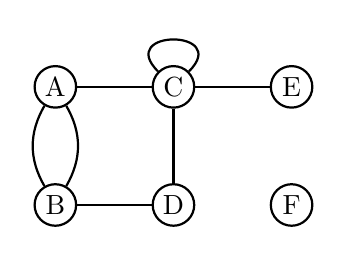
\begin{tikzpicture}[node distance={15mm}, thick, main/.style = {draw, circle}]
      \centering
      \tikzstyle{vertex}=[circle,draw=black,thick,fill=white,minimum size=15pt, inner sep=0pt]
      \node[vertex] (A) at (0, 0) {A};
      \node[vertex] (B) at (0, -1.5) {B};
      \node[vertex] (C) at (1.5, 0) {C};
      \node[vertex] (D) at (1.5, -1.5) {D};
      \node[vertex] (E) at (3, 0) {E};
      \node[vertex] (F) at (3, -1.5) {F};
      \path
      (A) edge (C)
      (C) edge [out=45,in=135,looseness=5] (C)
      (C) edge (E)
      (A) edge [bend left] (B)
      (A) edge [bend right] (B)
      (B) edge (D)
      (C) edge (D)
      ;
    \end{tikzpicture}
  \end{figure}
  We have \(deg(A) = 3,\ deg(B) = 3,\ deg(C) =5,\ deg(D) = 2,\ deg(E) = 1,\ deg(F) = 0\)  
\end{eg}

For a simple graph \(G\) with \(n\) vertices, if it is an undirected graph, we have a maximum of \(\binom{n}{2} = \frac{n(n-1)}{2}\) edges; if it is a directed graph, then we have a maximum of \(n(n-1)\) edges. 

\begin{eg}
  Prove the proposition: among 6 people, there will be '3 mutual acquaintances' or '3 mutual strangers'. Both can happen at the same time. 

  Consider a graph \(G = (V, E)\) where \(V\) is the set of people, and \(E\) indicates acquaintance. For example,
  \begin{figure}[H]
    \centering
    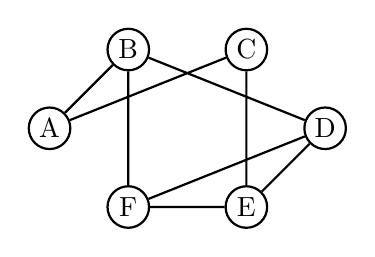
\begin{tikzpicture}[node distance={15mm}, thick, main/.style = {draw, circle}]
      \centering
      \tikzstyle{vertex}=[circle,draw=black,thick,fill=white,minimum size=15pt, inner sep=0pt]
      \node[vertex] (A) at (0, 0) {A};
      \node[vertex] (B) at (1, 1) {B};
      \node[vertex] (C) at (2.5, 1) {C};
      \node[vertex] (D) at (3.5, 0) {D};
      \node[vertex] (E) at (2.5, -1) {E};
      \node[vertex] (F) at (1, -1) {F};
      \draw
      (A) -- (B)
      (A) -- (C)
      (B) -- (F)
      (B) -- (D)
      (C) -- (E)
      (F) -- (D)
      (F) -- (E)
      (E) -- (D)
      ;
    \end{tikzpicture}
  \end{figure}
  For anyone in the graph, number of neighbors + number of non-neighbors = 5.
  By pigeonhole principle, we have at least \(\lceil \frac{5}{2} \rceil = 3\) neighbor or non-neighbors for a person.  

  \textbf{Case 1}: number of neighbors of A \(\geq 3\). Let \(B, C, D\) be the neighbors, i.e. 
  \begin{figure}[H]
    \centering
    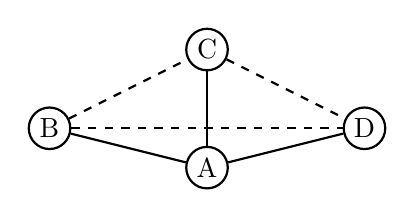
\begin{tikzpicture}[node distance={15mm}, thick, main/.style = {draw, circle}]
      \centering
      \tikzstyle{vertex}=[circle,draw=black,thick,fill=white,minimum size=15pt, inner sep=0pt]
      \node[vertex] (B) at (0, 0) {B};
      \node[vertex] (C) at (2, 1) {C};
      \node[vertex] (D) at (4,0) {D};
      \node[vertex] (A) at (2, -0.5) {A};
      \path
      (A) edge (B)
      (A) edge (C)
      (A) edge (D)
      (B) edge [dashed] (C)
      (B) edge [dashed] (D)
      (C) edge [dashed] (D)
      ;
    \end{tikzpicture}
  \end{figure}
  If \((B, C) \in E\) or \((C, D) \in E\) or \((B, D) \in E\), then we have a triangle formed by three nodes, i.e. there are three acquaintances. 

  If \((B, C) \notin E\) and \((C, D) \notin E\) and \((B, D) \notin E\), then we have three mutual strangers. 

  \textbf{Case 2}: number of non-neighbors of A \(\geq 3\). Let \(B, C, D\) be the non-neighbors, i.e. 
  \begin{figure}[H]
    \centering
    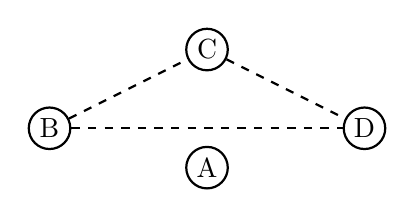
\begin{tikzpicture}[node distance={15mm}, thick, main/.style = {draw, circle}]
      \centering
      \tikzstyle{vertex}=[circle,draw=black,thick,fill=white,minimum size=15pt, inner sep=0pt]
      \node[vertex] (B) at (0, 0) {B};
      \node[vertex] (C) at (2, 1) {C};
      \node[vertex] (D) at (4,0) {D};
      \node[vertex] (A) at (2, -0.5) {A};
      \path
      (B) edge [dashed] (C)
      (B) edge [dashed] (D)
      (C) edge [dashed] (D)
      ;
    \end{tikzpicture}
  \end{figure}

  If \((B, C) \in E\) or \((C, D) \in E\) or \((B, D) \in E\), then we have a triangle formed by three nodes, i.e. there are three acquaintances. 

  Otherwise, \(A\) and at least 2 members from \(B, C, D\) will form a group of 3 mutual strangers.
\end{eg}